% \begin{savequote}[8cm]
% Alles Gescheite ist schon gedacht worden.\\
% Man muss nur versuchen, es noch einmal zu denken.

% All intelligent thoughts have already been thought;\\
% what is necessary is only to try to think them again.
%   \qauthor{--- Johann Wolfgang von Goethe \cite{von_goethe_wilhelm_1829}}
% \end{savequote}

% From the CIPS paper

\newcommand{\kcat}[0]{k_{\mathrm{cat}}}
\newcommand{\kspo}[0]{k_{\mathrm{spo}}}
\newcommand{\rcat}[0]{r_{\mathrm{cat}}}
\newcommand{\rspo}[0]{r_{\mathrm{spo}}}

\newcommand{\Rs}[0]{R_\mathrm{s}}
\newcommand{\Rp}[0]{R_\mathrm{p}}
\newcommand{\Ree}[0]{R_\mathrm{e}}

\newcommand{\phie}[0]{\phi_{\mathrm{e}}}
\newcommand{\phis}[0]{\phi_{\mathrm{s}}}
\newcommand{\phip}[0]{\phi_{\mathrm{p}}}
\newcommand{\phisp}[0]{\phi_{\mathrm{s+p}}}
\newcommand{\phiw}[0]{\phi_{\mathrm{w}}}

\newcommand{\mue}[0]{\mu_{\mathrm{e}}}
\newcommand{\muf}[0]{\mu_{\mathrm{f}}}
\newcommand{\mus}[0]{\mu_{\mathrm{s}}}
\newcommand{\mup}[0]{\mu_{\mathrm{p}}}
\newcommand{\muw}[0]{\mu_{\mathrm{w}}}

\newcommand{\Des}[0]{D_{\mathrm{es}}}
\newcommand{\Dse}[0]{D_{\mathrm{se}}}
\newcommand{\Dep}[0]{D_{\mathrm{ep}}}
\newcommand{\Dpe}[0]{D_{\mathrm{pe}}}
\newcommand{\Dsp}[0]{D_{\mathrm{sp}}}
\newcommand{\Dps}[0]{D_{\mathrm{ps}}}
\newcommand{\Dew}[0]{D_{\mathrm{ew}}}
\newcommand{\Dsw}[0]{D_{\mathrm{sw}}}
\newcommand{\Dpw}[0]{D_{\mathrm{pw}}}

\newcommand{\Mee}[0]{M_{\mathrm{ee}}}
\newcommand{\Mes}[0]{M_{\mathrm{es}}}
\newcommand{\Mep}[0]{M_{\mathrm{ep}}}
\newcommand{\Mse}[0]{M_{\mathrm{se}}}
\newcommand{\Mss}[0]{M_{\mathrm{ss}}}
\newcommand{\Msp}[0]{M_{\mathrm{sp}}}
\newcommand{\Mpe}[0]{M_{\mathrm{pe}}}
\newcommand{\Mps}[0]{M_{\mathrm{ps}}}
\newcommand{\Mpp}[0]{M_{\mathrm{pp}}}
\newcommand{\Mwp}[0]{M_{\mathrm{wp}}}
\newcommand{\Mws}[0]{M_{\mathrm{ws}}}
\newcommand{\Mwe}[0]{M_{\mathrm{we}}}


\newcommand{\vp}[0]{v_{\mathrm{p}}}
\newcommand{\vs}[0]{v_{\mathrm{s}}}
\newcommand{\ve}[0]{v_{\mathrm{e}}}
\newcommand{\vw}[0]{v_{\mathrm{w}}}

\newcommand{\ex}[1]{\mathrm{e}^{#1}}
\newcommand{\kb}[0]{k_{\rm B}}

\chapter{\label{ch:2-draft}Active Phase Separation of Dense Mixtures}

\minitoc
\newpage

\section{Introduction}

A lipid bilayer model with only one lipid component can undergo a melting transition, yet a lipid mixture can show phase coexistence, even with as little as two phospholipids and a cholesterol component \cite{elson_phase_2010}. Model cell membranes, made of these mixtures, result in regions of a liquid ordered and liquid disordered phase, and depending on the lipid composition, additional gel phases can also appear \cite{sych_how_2021, aufderhorst-roberts_three-phase_2017}. Lipid-lipid and lipid-cholesterol interactions can drive the well mixed system to form these separate domains, where the proportion of saturated and unsaturated lipids differ in each domain and the size of the domains can be either macroscopic or nanoscopic depending on composition \cite{feigenson_phase_2009}. Temperature dependent interactions built on equilibrium models of phase separating systems can predict the phase behaviour \cite{wolff_thermodynamic_2011}, however in these model systems the amount of lipid is conserved. In vivo, local lipid composition actually changes due to membrane recycling and as a result of the activity of enzymes which catalyse lipid synthesis and breakdown \cite{feigenson_phase_2009}. These features are not incorporated into existing theory, but could give rise to additional spatial organisation in living membranes.

Theoretical models describing the physics of of liquid-liquid phase separation have developed significantly in recent years, partly driven by the observation of membraneless organelles in vivo \cite{shin_liquid_2017}. A key development in the field has been to add non-equilibrium effects into descriptions of phase transitions including, actively propelled particles \cite{cates_motility-induced_2015}, phoretic transport effects \cite{agudo-canalejo_active_2019} and changes in chemical composition \cite{weber_drops_2021, li_non-equilibrium_2020}. The role of membranes and their interplay with phase separated droplets has also been an exciting area of research, through wetting and remodelling of vesicle membranes by liquid droplets \cite{mangiarotti_wetting_2023}. However this chapter focuses on the organisation of lipids in the plane of a membrane rather than coupling membrane effects to external droplets. In order to capture the effects of changes in composition, this chapter explores ideas from non-equilibrium phase transitions and develops a minimal model to describe an active mixture containing an enzyme component such as might be found from enzymes embedded in phospholipid bilayers \cite{alberts_molecular_2008}.

\section{Equilibrium Phase Separation}

\subsection{Thermodynamics of Fluid Mixtures}

A good example to explore the theory of phase separating mixtures is to study a fluid made up of two components, say, component $A$ and component $B$. To make this mixture, we mix $N_A$ molecules of component $A$ and $N_B$ molecules of component $B$ to give a mixture of total volume $V = v_A N_A + v_B N_B$, where $v_i$ is the specific volume of the component, the \textit{size} of each molecule. The volume fraction of a component, $\phi_i$, in some region of volume, $v$, is defined to be $\phi_i = v_i N_i/v$ and for the two component mixture with constant volume everywhere $\phi_A+\phi_B = 1$. To simplify the notation, let $\phi_A=\phi$ and $\phi_B=1-\phi$, and the volume fraction $\phi$ now describes the proportion of the fluid volume that is component $A$. For an incompressible fluid, the total volume is constant and the relevant free energy is the Helmholtz free energy, $F(N_A, N_B, T)$ where $T$ is the temperature of the fluid. The Helmholtz Free energy is an extensive quantity and so for a homogeneous mixture $F(N_A, N_B, T) = V f(\phi, T)$ where $f(\phi, T)$ is the free energy density and this free energy density determines the phase behaviour of the mixture. If a system phase separates into two coexisting phases, then the free energy of two phase system is $V_{\mathrm{I}} f(\phi_{\mathrm{I}}, T)+ V_{\mathrm{II}} f(\phi_{\mathrm{II}}, T)$ where the two phases are labelled $\mathrm{I}$ and $\mathrm{II}$ and the total volume of the system is conserved $V = V_{\mathrm{I}}+V_{\mathrm{II}}$. It is necessary for the two phase free energy to be lower than the free energy of an equivalent homogeneous system in order for the system to phase separate \cite{jones2002soft}.

In addition to lowering the free energy of the system, any phase separating regions of a mixture must also be in mechanical and chemical equilibrium, otherwise they would exchange components or volume to reach two equilibrated phases. Chemical equilibrium is achieved when the chemical potential, $\mu$ of each component in each phase is constant and so moving a particle across the phase boundary will not change the free energy, $\mu_i^{\mathrm{I}}=\mu_i^{\mathrm{II}}$. The chemical potential for component $i$ is given by
\begin{equation}
    \mu_i = \left(\frac{\partial F}{\partial N_i}\right)_{V, T} = v_i \left(\frac{\partial f}{\partial \phi_i}\right)_{T}.
    \label{eq:2-mu_def}
\end{equation}
The mechanical equilibrium is achieved when the osmotic pressure, $\Pi$ between the two phases is equal, $\Pi^{\mathrm{I}}=\Pi^{\mathrm{II}}$, where the osmotic pressure is given by
\begin{equation}
    \Pi(\phi) = -\left(\frac{\partial F}{\partial V}\right)_{T, N_A} = -f + \phi \left(\frac{\partial f}{\partial \phi}\right)_{T}.
    \label{eq:2-Pi_def}
\end{equation}
since $\phi = N_A v_a/V$ and so $\frac{\partial \phi}{\partial V} = -\phi/V$ \cite{doi_soft_2013}. These conditions have a convenient graphical interpretation. The equation for a tangent to the curve $f(\phi)$ at $\phi=\Tilde{\phi}$ can be written as $y=mx+c$. Equations (\ref{eq:2-mu_def}) and (\ref{eq:2-Pi_def}) give $y=\mu_A(\Tilde{\phi})\phi - \Pi(\Tilde{\phi})$ and as these thermodynamic quantities must be the same for two coexisting phases, we find that two phases can only coexist if they have a \textit{common tangent}! Figure \ref{fig:phase_sep_scheme} highlights the graphical interpretation of these conditions, where plotting $f(\phi)$ can illuminate the phase behaviour of a mixture. A well mixed homogeneous system prepared with volume fraction $\phi^*$, will therefore be stable as two phase separated with regions volume fraction $\phi_{\mathrm{I}}$ and $\phi_{\mathrm{II}}$ ($\phi_{\mathrm{I}} < \phi_{\mathrm{II}}$) given that $\phi_{\mathrm{I}} < \phi^* < \phi_{\mathrm{II}}$ \cite{weber2019physics}. The conservation of $N_A$ requires $V\phi^* = V_{\mathrm{I}}\phi_{\mathrm{I}} +V_{\mathrm{II}}\phi_{\mathrm{II}}$ and volume conservation gives $V = V_{\mathrm{I}}+V_{\mathrm{II}}$ which determines the volumes of each phase

\begin{equation}
    V_{\mathrm{I}} = \frac{\phi_{\mathrm{II}}-\phi^*}{\phi_{\mathrm{II}}-\phi_{\mathrm{I}}}V
    \quad
    \textrm{and}
    \quad
    V_{\mathrm{II}} = \frac{\phi^*-\phi_{\mathrm{I}}}{\phi_{\mathrm{II}}-\phi_{\mathrm{I}}}V.
\end{equation}

\begin{figure}
    \centering
    \includegraphics[width=\textwidth]{figures/thermo_solutions.pdf}
    \caption{Schematic of equilibrium phase separation, showing a system that exhibits coexisting phases at some temperature $T_{A}$, but not at another temperature $T_{B}$ which has a convex free energy. In the lower plot examples of the distribution of the two phases in a system are shown with two examples of a phase separated system.}
    \label{fig:phase_sep_scheme}
\end{figure}

Often, the shape of the free energy density can be controlled by some external parameter, such as temperature. When the temperature and consequently the free energy is changed, the two volumes fraction of the coexisting phases also changes. Calculating the the two phases ($\phi_{\mathrm{I}}$ and $\phi_{\mathrm{II}}$) as the temperature changes sweeps out a loci of points called the binondal curve. This is shown graphically in figure \ref{fig:bino_spino_scheme}.

Another important feature of a free energy landscape is the spinodal curve. This curve defines the region where the free energy is unstable, $\frac{\partial^2 f}{\partial \phi^2} > 0$. As such, a mixture in the spinodal region is unstable to small perturbations and will decay into the phase separated state spontaneously. There also exists a region in between the spinodal and binodal curves that is metastable: the free energy would be lower in a phase separated system, but there is an energy barrier preventing the system from transitioning to this state. A large enough pertubation, for example from temperature fluctuations could overcome this nucleation barrier, but often in real systems imperfections, or external structures, can act as nucleation sites and cause the transition. This region is also shown in figures \ref{fig:phase_sep_scheme} and \ref{fig:bino_spino_scheme}, where the shaded region is the unstable spinodal region and the boundary defines the spinodal curve \cite{jones2002soft}.

\begin{figure}
    \centering
    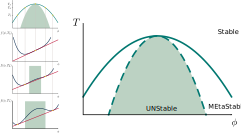
\includegraphics[width=0.9\textwidth]{figures/bino_spino_scheme.pdf}
    \caption{Graphical explanation of how the phase diagram for an equilibrium system is calculated. The solid, binodal line is the boundary between the stable and metastable state and the dashed spinodal line is the boundary between the unstable and metastable states. The two lines meet at the critical point.}
    \label{fig:bino_spino_scheme}
\end{figure}


\subsection{Regular Solution Model}
Mean field models of mixtures can describe the free energy density and predict features of the phase behaviour. Coarse grained order parameters, such as volume fractions provide a useful description of the system, where the volume fraction describes the local  composition, but may not be homogeneous in the system. These order parameters describe the dynamics of an intermediate scale, much larger than the individual lattice sites and much smaller than the overall system size.
The free energy density can be calculated from the Hamiltonian of a system and, again, the $A-B$ binary mixture is a useful place to start. Consider a lattice where each lattice site is occupied by either a molecule of $A$ or a molecule of $B$ where $v_A$ and $v_B$ (the size of each molecule) is the same and is equal to one lattice site. The total number of sites in the lattice  is $N_{lat} = N_A + N_B$. The different molecules can be configured in many different ways on the lattice however the different configurations will have different energies due to interactions between the molecules. The lattice model can include these interactions by having different contributions to the energy for different pairs of molecules on neighbouring lattice sites. For example, two molecules of $A$ on neighbouring sites will contribute $\epsilon_{AA}$ to the energy of a configuration, two molecules of $B$ contribute $\epsilon_{BB}$ and a molecule of $A$ on a neighbouring lattice site to a molecule of $B$ will contribute $\epsilon_{AB}$. The total energy of a configuration $c$ is then the sum of the interaction energy contribution over all neighbouring lattice sites
\begin{equation}
    E_{c} = N_c^{AA}\epsilon_{AA} + N_c^{AB}\epsilon_{AB} + N_c^{BB}\epsilon_{BB}
\end{equation}
where $N_c^{ij}$ is the number of neighbouring lattice site pairs, occupied by a molecule of $i$ and molecule of $j$ in the configuration. The free energy desnity can be calculated from the partition function, $Z$, as
\begin{equation}
    f(\phi, T) = -\frac{\kb T}{V}\ln Z
    \label{eq:2-f_ln}
\end{equation}
where $\kb$ is the Boltzmann constant \cite{kardar2007statistical}. The partition function is directly calculated for a canonical ensemble via
\begin{equation}
    Z = \sum_c \exp{(-\beta E_c)}.
\end{equation}
where $\beta = 1/\kb T$ and the sum is over all configurations. In the thermodynamic limit of large $N_{lat}$ the sum can be well approximated by a mean field approximation. The sum is approximated by replacing the energy of each configuration with the average energy, $\bar{E}$, so the sum now becomes
\begin{equation}
    Z \approx \sum_c \exp(-\beta \bar{E}) = \Omega \exp(-\beta \bar{E})
\end{equation}
where $\Omega$ is the number of unique configurations of molecules on the lattice and is given by
\begin{equation}
    \Omega = \frac{N_{lat}!}{N_A! N_B!}.
\end{equation}

The free energy density in the mean field model is now, with equation (\ref{eq:2-f_ln}), $f = -\frac{K_B T}{V} (\ln \Omega + \bar{E})$.

The mean energy $\bar{E}$ can be calculated in the mean field model. The coordination number, $z$, describes the number of nearest neighbours of each lattice site, for example $z=4$ in a square lattice. On average $z\phi_i$ of the neighbouring lattice sites will be occupied by a molecule of $i$. For $i \neq j$ the average number of $ij$ neighbour pairs, $\bar{N}^{ij}$, is the number of sites occupied by a molecule of $i$ multiplied by the average the number of neighbouring lattice sites occupied by a molecule of $j$: $\bar{N}^{ij} = N_{lat}\phi_i \times z\phi_j$. When $i=j$ each pair will be double counted (each lattice site occupied by a molecule of $i$ will be considered as both the `main' and `neighbour' site) and so there is an additional factor of 1/2 to prevent double counting \cite{doi_soft_2013}. The average energy is therefore
\begin{equation}
\begin{split}
    \bar{E} &= \bar{N}^{AA}\epsilon_{AA} + \bar{N}^{AB}\epsilon_{AB} + \bar{N}^{BB}\epsilon_{BB}\\
    &= \frac{1}{2}z N_{lat} \phi^2\epsilon_{AA} + z N_{lat} (1-\phi)\phi\epsilon_{AB} + \frac{1}{2}z N_{lat} (1-\phi)^2 \epsilon_{BB}.
\end{split}
\end{equation}
Using equation (\ref{eq:2-f_ln}) the free energy density is
\begin{equation}
    f(\phi, T) = -\frac{\kb T}{V}\left(\ln \left(\frac{N_{lat}!}{N_A! N_B!} \right) - \frac{z N_{lat}}{2} \left(\phi^2\epsilon_{AA} + 2(1-\phi)\phi\epsilon_{AB} + (1-\phi)^2 \epsilon_{BB}\right)\right).
\end{equation}
The first term is simplified using Stirling's formula, $\ln N! = N \ln N - N$ for large $N$ to give $\ln\Omega=-N_{lat}(\phi\ln(\phi)+(1-\phi)\ln(1-\phi))$. The average energy term can be simplified as the phase behaviour is independent of the exact value of $f$, or $\partial f/\partial \phi$ and so the physics of the system is symmetric under a transform $f \rightarrow f + k_1 + k_2\phi$. Specifically, choosing $k_1 = z\epsilon_{BB}/2$ and $k_2 = z(\epsilon_{BB} - \epsilon_{AA})/2$ the free energy now becomes
\begin{equation}
    \frac{f(\phi, T)}{\kb T} = \phi\ln(\phi)+(1-\phi)\ln(1-\phi) + \chi(1-\phi)\phi
    \label{eq:2-fh_free}
\end{equation}
since $V = N_{lat}$ and define the Flory-Huggins interaction parameter $\chi = -\frac{z}{2 k_B T} (\epsilon_{AA} + \epsilon_{BB} - 2\epsilon_{AB})$, which is the energy change when a molecule of A is taken from an environment of pure A and put into an evnironment of pure B --- for $\chi<0$ it is energetically favourable for the components to mix and for $\chi>0$ it is favourable for the components to remain separate. The spinodal region can be found by directly calculating the $\frac{\partial^2f}{\partial\phi^2}$ and this shows the existence of a critical point at $\phi_\text{crit}=0.5$ and $\chi_\text{crit}=2$ and so for $\chi<2$ the system cannot phase separate. The critical point must occur $\phi_\text{crit}=0.5$ as the system is symmetric under exchange of $A, B \rightarrow B, A$, however the homogeneous system can be stable for all $\phi$ even when mixed interactions are unfavourable $\chi>0$. This is because when $0<\chi<2$, the entropic terms in the free energy contribute more than the cost of the interactions and so the system remains stable. In equilibrium theories of phase separation it is the interactions that drive the phase behaviour.

\subsubsection{Generalisations of the Regular Solution Free Energy}

The Flory-Huggins theory gives the free energy of a binary mixture in equation (\ref{eq:2-fh_free}), however a similar form of the free energy can be extended to describe a broader class of mixtures. Consider a system of $N$ components, where the mixture is made up of volume fraction $\phi_i$ of component $i$ and $i$ runs from $1$ to $N$. In a system with non-conserved particle number (such as an active system discussed later) the free energy will have additional enthalpic terms. This is intrinsic energy from chemical bonds in a molecule of each species and this contributes linearly in volume fraction to the free energy to give
\begin{equation}
    f_\text{enth} = \sum_{i}\varepsilon_i \frac{\phi_i}{v_i}
\end{equation}
where $\varepsilon_i$ is the enthalpy per molecule of component $i$. If different components in the system have molecules that occupy more than one lattice site, then the previous calculation of $\Omega$, the number of microstates, is overestimated, as nearby sites will necessarily be occupied by the same molecule. This modifies the entropic contribution to the free energy and the Flory-Huggins theory gives the entropic contribution as
\begin{equation}
    f_\text{entr} = \sum_{i}\kb T \frac{\phi_i}{v_i}\ln\phi_i
\end{equation}
as if a molecule is larger, then there are fewer molecules per volume and therefore fewer microstates. Volume effects will also appear in the calculation of the chemical potential, due to the conversion between volume fraction and the number of molecules
\begin{equation}
    \mu_i = \frac{\partial F}{\partial N_i} = v_i\frac{\partial F}{\partial \phi_i}.
\end{equation}
For a mixture of $N$ components the full theory will describe interactions between all components so that the contribution to the free energy from interactions becomes
\begin{equation}
    f_\text{int} = \sum_{i, j}\frac{\chi_{ij}}{2}\phi_i\phi_j.
\end{equation}
where the sum denotes the double sum running from $0$ to $N$ for both indices, the factor of $1/2$ means each interaction is only counted once and the scalar interaction parameter, $\chi$, has now become a matrix of interaction parameters, $\chi_{ij}$ \cite{mao_phase_2019}. Noting incompressibility, $\sum_{i}\phi_i = 1$, gives
\begin{equation}
\begin{split}
    f_\text{int} &= \sum_{i, j}\frac{\chi_{ij}}{2}\phi_i\phi_j = \sum_{i}\left(c_i\phi_i-\left(\sum_j c_i\phi_i\phi_j\right)\right) + \sum_{i, j}\frac{\chi_{ij}}{2}\phi_i\phi_j \\
    &= \sum_{i}c_i\phi_i + \sum_{i,j}\left(\frac{\chi_{ij}}{2}-c_i\right)\phi_i\phi_j.
\end{split}
\end{equation}
Defining $\tilde{\chi}_{ij}=\chi_{ij}-2c_i$ and choosing $c_i = \chi_{ii}/2$ eliminates the diagonal term so the $\tilde{\chi}_{ii} = 0$ for all $i$. This term can be contained into a modified enthalpic term which includes the intrinsic enthalpy and self interactions $\tilde{\varepsilon_i} \rightarrow \varepsilon_i + \chi_{ii/2}$. Since the free energy can be written in terms of these modified enthalpic terms and interaction terms, it is convenient to immediately drop the tildes and write the free energy using an interaction parameter with zeros on the diagonal.

The final contribution considered here describes an energy of interfaces and is related to the surface tensions between domains of different compositions. Similarly to the interaction term, in the case of an $N$ component matrix, the interface contribution to the free energy will be composed of couplings between the gradient of the volume fractions of each component with each other to give
\begin{equation}
    f_\text{surf} = \sum_{i, j}\frac{\kappa_{ij}}{2}(\nabla\phi_i)\cdot(\nabla\phi_j)
\end{equation}
where $\kappa$ is an $N \times N$ matrix that recovers the surface tension in the system. Another consequence of incompressibility is $\sum_{i}\nabla\phi_i = 0$ and so
\begin{equation}
\begin{split}
    f_\text{surf} &= \sum_{i,j}\frac{\kappa_{ij}}{2}\left(\nabla\phi_i\right)\cdot\left(\nabla\phi_j\right) = \sum_{i,j}\frac{\kappa_{ij}}{2}\left(\nabla\phi_i\right)\cdot\left(\nabla\phi_j\right) - \sum_{i}\nabla\phi_i\cdot\left(\sum_j b_i\nabla\phi_j\right) \\
    &= \sum_{i,j}\left(\frac{\kappa_{ij}}{2} - b_i \right)\left(\nabla\phi_i\right)\cdot\left(\nabla\phi_j\right)
\end{split}
\end{equation}
where setting $2b_i = \kappa_{ij}$ shows that the gauge of the system can be chosen such that $\kappa_{ii} = 0$. Additional terms that go like higher power gradient terms, or external potentials can be added to the free energy, however these ingredient capture all features of the classical theories of phase separation and the resulting dynamics.

The overall Flory Huggins free energy density, $f_\text{FH}$, is therefore
\begin{equation}
    f_\text{FH} = \sum_{i=1}^{N}\Bigg[\frac{\phi_i}{v_i}(\ln\phi_i+\varepsilon_i)+\sum_{j=1, j\neq i}^{N}\frac{\chi_{ij}}{2}\phi_i\phi_j + \sum_{j=1, j\neq i}^{N} \frac{\kappa_{ij}}{2}(\nabla\phi_i)\cdot(\nabla\phi_j)\Bigg].
    \label{fh_gen}
\end{equation}

\section{Dynamics of Multi-component mixtures}

\subsection{Conserved Dynamics}

\subsubsection{Model B Dynamics}
The static lattice picture can describe the free energy of a system, but, alone, does not describe associated dynamics. The lattice model can be extended to include the evolution of a system through configuration space by considering exchange of molecules of neighbouring lattice sites. In this picture (and also physically), the number of molecules of each species does not change and so the behaviour of the volume fraction for each component must obey a continuity equation, namely\cite{li_non-equilibrium_2020}
\begin{equation}
    \dot{\phi}_i = - \nabla \cdot \textbf{J}_i
    \label{eq:2-continuityModB}
\end{equation}
where $i$ labels each component, and $\textbf{J}_i$ is the volume fraction flux. Assuming near equilibrium linear response \cite{groot_non-equilibrium_1984}, changes to the distribution of a component will be driven by changes in the free energy and the associated thermodynamic force, specifically the chemical potential. The canonical Model B dynamics capture this chemical pressure and give the volume fraction flux as
\begin{equation}
    \textbf{J}_i = \sum_j M_{ij}\nabla\mu_j + \textbf{J}^N
    \label{eq:2-fluxModB}
\end{equation}
where $\mu_i$ is the chemical potential of the $i\th$ component, $M_{ij}$ is a set of generalised mobilities and the sum runs over all components in the system \cite{hohenberg_theory_1977, li_non-equilibrium_2020}. The $\textbf{J}^N$ term describes the noise and must obey the appropriate fluctuation dissipation theorems. In the thermodynamic limit of a noise free model considered here the $ \textbf{J}^N$ contribution vanishes. The chemical potential for each component, $\mu_i$, is given by
\begin{equation}
    \mu_i = v_i\frac{\delta F}{\delta \phi_i}.
\end{equation}
where the functional derivative is used since $\phi_i$ depends on position.

\subsubsection{Mobilities for Incompressible Models} \label{subsec:mob}

The model B dynamics introduce a set of transport coefficients, or mobilities $M_{ij}$, which describe how volume fraction of the $i\th$ component responds to the chemical potential of the $j\th$ component. This is a general form of linear transport relationship found near equilibrium in thermodynamic systems where fluxes are proportional to a set of generalised conjugate thermodynamic forces $J_i = \sum_{j}L_{ij}\nabla f_{j}$. In this generalised description, the transport coefficient matrix described by $L_{ij}$ is both positive semi-definite (positive entropy production rate) and symmetric under exchange of $i, j \rightarrow j, i$. Here however, the flux describes the transport of volume fraction rather than particle number and so the the forces and displacements are not conjugate \cite{groot_non-equilibrium_1984}. As such the reciprocity is broken and $L_{ij} \neq L_{ji}$, however again using the size of individual molecules to convert between volume fraction and number density gives
\begin{equation}
    {M}_{ij} = \frac{v_i}{v_j}{M}_{ji}.
    \label{eq:2-mobsym}
\end{equation}

An incompressible model requires $\sum_i\phi_i = 1$ and so $\sum_i\dot{\phi}_i = 0$. Substituting in the Model B dynamics, equations (\ref{eq:2-continuityModB}) and (\ref{eq:2-fluxModB}) give
\begin{equation}
    \sum_i\dot{\phi}_i = \sum_i\;\nabla\cdot\bigg(\sum_j M_{ij}\nabla\mu_j\bigg) = \sum_j\;\nabla\cdot\bigg(\big(\sum_i M_{ij}\big)\nabla\mu_j\bigg) = 0.
\end{equation}
In order for this to be true in general, for non-uniform systems, i.e. $\nabla\mu_j \neq 0$, it is necessary for the mobilities to satisfy
\begin{equation}
    \sum_i M_{ij} = 0
    \label{eq:2-mobinc}
\end{equation}
which constrains the mobilities and enforces the fluid remains incompressible.\cite{kehr_mobility_1989} An $N$-component mixture,  has a total of $N\times N$ mobilities. The reciprocity-like constraint in equation (\ref{eq:2-mobsym}) reduces the number of free parameters to $N(N+1)/2$ and the incompressibility condition adds a further $N$ constraints to give $N(N-1)/2$ free mobility parameters.

\subsection{Non-Conserved Dynamics}

\subsubsection{Reaction Rates}
In addition to spatial fluxes of component from the Model B dynamics, chemically active mixtures will also permit fluxes in chemical space, i.e. the conversion of a molecule of $i$ to a molecule of $j$. Putting these dynamics into the binary mixture, we allow the reaction $A \rightleftharpoons B$, and an immediate consequence of incompressibility is that the reaction must conserve volume, so here $v_A = v_B$. In general the volume of the reactants must equal the volume of the products which is simple for this 1:1 stoichiometry but could be more complex for non-conserved molecule number. The change in the free energy due to the reaction is $dF = \mu_A dN_A+\mu_B dN_B = (\mu_A - \mu_B)dN_A$ where $dN_A = -dN_B$ by conservation of total molecule number. There is therefore no net conversation between molecules of $A$ and $B$ when $\mu_A = \mu_B$. Considering detailed balance \cite{weber_drops_2021} for the system constrains the relationship between the forward and backward reaction rates
\begin{equation}
    \frac{r_{A \rightarrow B}}{r_{B \rightarrow A}} = \exp\Bigg(\frac{\mu_A - \mu_B}{k_B T}\Bigg)
    \label{db_constr}
\end{equation}
which allows us to identify the net transfer from $A \rightarrow B$ as
\begin{equation}
    r_{A \rightarrow B} - r_{B \rightarrow A} = K\Bigg(\exp\bigg(\frac{\mu_A - \mu_B}{k_B T}\bigg)-1\Bigg).
    \label{eq:2-sponrate}
\end{equation}
This makes sense as if $\mu_A > \mu_B$ then we have net $A \rightarrow B$, when $\mu_B > \mu_A$ then we have net $B \rightarrow A$ and as expected there is no net flux for $\mu_A = \mu_B$ \cite{weber2019physics}.

\subsubsection{Enzymatic Activity}
Enzymes act as catalysts in biological reactions and increase the rate of a reaction. This can be achieved by the presence of an active site that allows a fuel driven reaction, or for the reaction to occur via some alternative route that can only happen in the presence of this \textit{enzyme} component. This can be modelled as the reaction now occurring as
\begin{equation}
    \text{Enzyme + Fuel} + A \leftrightharpoons \text{Enzyme + Waste} + B
\end{equation}
where the system is in contact with a Fuel and Waste reservoir that maintains constant chemical potentials, $\mu_{Fuel}$ and $\mu_{Waste}$, and define $\Delta\mu \equiv \mu_{Fuel}-\mu_{Waste}$ which is also constant. Alternatively, $\Delta \mu$ could represent the energy transferred by a photon in a light-activated catalytic reaction. Using equation (\ref{db_constr}) the rate of $A \rightarrow B$ of this reaction in the presence of the enzyme can be written as
\begin{equation}
    r_{A \rightarrow B,E} - r_{B \rightarrow A,E} = K'\rho_\textrm{E}\Bigg(\exp\bigg(\frac{\mu_A - \mu_B + \Delta\mu}{k_B T}\bigg)-1\Bigg)
    \label{eq:2-enzrate}
\end{equation}
where the reaction rate is proportional to the local concentration of the enzyme component, $\rho_\textrm{E}$, and $K'$ is the modified rate constant. Reaction kinetics of enzymes are often described using Michaelis–Menten kinetics with $r_{A\rightarrow B}\sim\rho_\textrm{E}\rho_\textrm{A}/(K_{M}+\rho_\textrm{A})$ where $K_M$ is the Michaelis constant and $\rho_\textrm{A}$ is the concentration of the substrate, A \cite{murray_mathematical_1993}. In both  descriptions of the kinetics, the rate increases linearly with $\rho_\textrm{E}$ however, equation (\ref{eq:2-enzrate}) will additionally capture the effect of interactions on the rate of conversion when compared to the Michaelis-Menten rate.

\section{Minimal Model of an Active Mixture}

The simplest model that will encapsulate all of these effects requires at least two components for a chemical reaction to occur, e.g. $S \rightleftharpoons P$ (substrate to product) and a third enzyme component (E), that permits the driven, catalytic reaction described in equation (\ref{eq:2-enzrate}). At every point in space and time system is parameterised by three volume fractions; $\phis(\bm{r},t)$, $\phip(\bm{r},t)$ and $\phie(\bm{r},t)$, corresponding to individual molecules of volume $\vs$, $\vp$ and $\ve$ respectively. The mixture is incompressible and so $\phis+\phip+\phie=1$ everywhere and consequently the reaction requires, $\vs = \vp$. In living systems, enzymes have much more complex structures than reactants and so we expect the size of this component to be much larger $\ve > \vs, \vp$ \cite{berg_biochemistry_2002}. This increased size is also expected to result in increased viscous drag and reduced mobility for an enzyme compared to the other components. The Flory-Huggins theory of suspensions gives the free energy of the system as $F = \int \mathrm{d}\bm{r} f_\mathrm{FH}$, with the free energy density
\begin{equation}
    f_\mathrm{FH}(\{\phi_i\}) = \sum_{i=1}^{N} \frac{1}{v_i} \big[\varepsilon_i\phi_i + k_\mathrm{B}T \phi_i \log\phi_i \big], 
    \label{eq:2-fh_gen}
\end{equation}
where $\varepsilon_i$ is the enthalpy of component $i$. Importantly, we do not include any interaction terms in the free energy, in particular $f_\mathrm{FH}$ does not contain terms of the usual form $\chi_{ij}\phi_i \phi_j$. This implies that phase separation in this system would be impossible at equilibrium. The chemical potential of a component is given by
\begin{equation}
    \mu_i = e_i + \log\phi_i + 1 \quad \text{and so} \quad \nabla\mu_i = \frac{1}{\phi_i}\nabla\phi_i
    \label{eq:2-chempot}
\end{equation}
which drive the conserved dynamics of Model B. For the mobilities we assume the common form where $M_{ij} = -\beta D_{ij}\phi_i\phi_j$ for $i \neq j$ and $\beta \equiv (k_\mathrm{B}T)^{-1}$ \cite{KRAMER1984473}. The mobility constraints imply $M_{jj}= - \sum_{i\neq j} M_{ij}$ and $v_j D_{ij} = v_i D_{ji}$ \cite{kehr_mobility_1989, mao_designing_2020, bo_stochastic_2021}. The transport coefficients $D_{ij}$ determine the rate at which the components respond to local effective concentration gradients and exchange positions, and as such are inherently related to the phenomena of diffusiophoresis, cross-diffusion and Maxwell-Stefan diffusion.

We make the model active by allowing non-equilibrium (fuelled) conversion between two components, substrate (S) and product (P), catalyzed by an enzyme (E). This can be described by the reaction E+S+F $\rightleftharpoons$ E+P+W, where F and W represent fuel and waste molecules, respectively. We do not model the dynamics of the fuel and waste here, but assume that the system is in contact with a reservoir that maintains constant chemical potentials, $\muf$ and $\muw$, and define $\Delta\mu \equiv \muf-\muw$. The catalysed reaction converts substrate to product with rate $\rcat$ and we also model the spontaneous reaction (does not require enzyme) which converts substrate to product at rate $\rspo$ (note that these contributions might be negative as this flux is always expressed in the direction $S \rightarrow P$). Evaluating equations (\ref{eq:2-sponrate}) and (\ref{eq:2-enzrate}) with the chemical potential from equation (\ref{eq:2-chempot}) gives
\begin{align}
    \rspo &= \rspo^{\mathrm{S}\to\mathrm{P}} - \rspo^{\mathrm{P}\to\mathrm{S}} = \kspo[e^{\beta \Delta \varepsilon}\phis - \phip],
    \label{eq:2-r_spo} \\
    \rcat &= \rcat^{\mathrm{S}\to\mathrm{P}} - \rcat^{\mathrm{P}\to\mathrm{S}} = \kcat\phie[\phis-\phip e^{-\beta(\Delta \varepsilon+ \Delta\mu)}],
    \label{eq:2-r_cat}
\end{align}
where $\Delta e = e_S - e_P$. The rate constants here have been scaled to better disentangle the effects of the various parameters; $k_{spo} = K_{spo}/\phi_P$ and $k_{cat} = K_{cat}e^{-(\Delta e + \Delta \mu)}/(\ve \phi_P)$. We will typically take $\Delta \varepsilon<0$ and $\Delta \varepsilon + \Delta \mu>0$, so that the spontaneous and catalyzed reactions run preferentially in the P$\to$S and S$\to$P directions, respectively.

Combining the conserved and non-conserved dynamics and defining $R\equiv\rspo+\rcat$ results in the evolution equations for the three-component system
\begin{align}
    \dot{\phie} &= \bm{\nabla} \cdot \big(\Mee\bm{\nabla}\mue + \Mes\bm{\nabla}\mus + \Mep\bm{\nabla}\mup\big), \label{eq:2-evoE}\\
    \dot{\phis} &= \bm{\nabla} \cdot \big(\Mse\bm{\nabla}\mue + \Mss\bm{\nabla}\mus + \Msp\bm{\nabla}\mup\big) - R, \label{eq:2-evoS}\\
    \dot{\phip} &= \bm{\nabla} \cdot \big(\Mpe\bm{\nabla}\mue + \Mps\bm{\nabla}\mus + \Mpp\bm{\nabla}\mup\big) + R. \label{eq:2-evoP}
\end{align}

\section{Catalysis Induced Phase Separation}
\subsection{Stability of the Homogeneous Steady State}
The minimal model in equations (\ref{eq:2-evoE})--(\ref{eq:2-evoP}) have a homogeneous steady-state solution when $R=0$. Since the enzyme component is conserved in the system we can define $\phie^*$ as the average enzyme volume fraction in the initialisation of a system, such that the total volume of enzyme component in the system is $V \times \phie^*$. For any $\phie^*$, solving $R=0$ gives steady state volume fraction for the substrate and product components
\begin{align}
    \phis^* &= \phisp^*\frac{\kspo + \kcat\phie^*e^{-\beta(\Delta \varepsilon + \Delta\mu)}}{\kspo + \kcat\phie^*e^{-\beta (\Delta \varepsilon + \Delta\mu)}+\kspo e^{\beta \Delta \varepsilon} + \kcat\phie^*}
    \label{eq:2-sstar}
    \\
    \phip^* &= \phisp^*\frac{\kspo e^{\beta \Delta \varepsilon} + \kcat\phie^*}{\kspo + \kcat\phie^*e^{-\beta (\Delta \varepsilon + \Delta\mu)}+\kspo e^{\beta \Delta \varepsilon} + \kcat\phie^*}
    \label{eq:2-pstar}
\end{align}
with $\phisp^*=1-\phie^*$, which is the average volume fraction of the substrate and product combined $(\phisp^*=\phis^*+\phip^*)$ and is also conserved.

We can study the linear stability of this homogeneous steady-state by considering a small perturbation $\phi_i(\bm{r},t) = \phi_i^* + \delta\phi_i(\bm{r}, t)$, giving $\mu_i(\bm{r},t) = \mu_i^* + \delta\mu_i(\bm{r},t)$ and define mobilities at the homogeneous steady state $M^*_{ij} = M_{ij}(\phie^*, \phis^*, \phip^*)$. To first order in the perturbation $\delta\mu(\bm{r},t) = \frac{\delta\phi_i(\bm{r},t)}{\phi_i^*}$ and thus $\bm{\nabla}\mu_i(\bm{r},t) = \frac{1}{\phi_i^*}\bm{\nabla}\delta\phi_i(\bm{r},t)$. Additionally, define how the reaction rate changes under a small change in $\phi_i$ to be $R_i$, such that $R = \Rs \delta \phis - \Rp \delta \phip + \Ree \delta \phie$ where the sign changes for the product component to keep $\Rp > 0$. This gives
\begin{align}
    \Rs &\equiv \kspo e^{\beta \Delta \varepsilon} + \kcat\phie^* \\
    \Rp &\equiv \kspo + \kcat\phie^*e^{-\beta (\Delta \varepsilon+\Delta \mu)} \\
    \Ree &\equiv k_\mathrm{cat} [ \phis^* - \phip^* e^{-\beta (\Delta \varepsilon + \Delta \mu)}] = \phi^*_\mathrm{s+p} \frac{k_\mathrm{cat} k_\mathrm{spo} (1-e^{-\beta \Delta \mu})}{k_\mathrm{spo} + k_\mathrm{cat} \phie^* e^{-\beta (\Delta \varepsilon + \Delta \mu)} + k_\mathrm{spo} e^{\beta \Delta \varepsilon} + k_\mathrm{cat} \phie^* }.
\end{align}
The governing equations for the perturbations $\delta\phi_i (\bm{q},t) $ in Fourier space are found as follows
\\
\noindent
\makebox[\textwidth]{\parbox{1.3\textwidth}{%
\begin{equation}
\begin{pmatrix}
\dot{\delta\phie}\\
\dot{\delta\phis}\\
\dot{\delta\phip}\\
\end{pmatrix} =
\underbrace{
\begin{pmatrix}
(\Mse^*+\Mpe^*)\frac{\bm{q}^2}{\phie^*} & -\Mse^*\frac{\ve}{\vs}\frac{\bm{q}^2}{\phis^*} & -\Mpe^*\frac{\ve}{\vs}\frac{\bm{q}^2}{\phip^*}\\
-\Mse^*\frac{\bm{q}^2}{\phie^*} - \Ree  & \big(\Msp^* + \Mse^*\frac{\ve}{\vs}\big)\frac{\bm{q}^2}{\phis^*} - \Rs  & -\Msp^*\frac{\bm{q}^2}{\phip^*} + \Rp \\
-\Mpe^*\frac{\bm{q}^2}{\phie^*}  + \Ree  & -\Msp^*\frac{\bm{q}^2}{\phis^*} + \Rs  & \big(\Mpe^*\frac{\ve}{\vs}+\Msp^*\big)\frac{\bm{q}^2}{\phip^*} - \Rp \\
\end{pmatrix}
}_{\cal C}
\begin{pmatrix}
\delta\phie\\
\delta\phis\\
\delta\phip\\
\end{pmatrix}.
\end{equation}}}
In this formulation, we can explicitly see the incompressibility being imposed as the columns of $\cal C$ sum to zero.
We now eliminate one of the components, e.g. $\delta\phip = -\delta\phie - \delta\phis$, and define a $2\times2$ matrix, $\cal K$, describing the evolution of the remaining components. This is obtained from $\cal C$ by subtracting the last column from the other two (i.e. ${\cal K}_{ij} = {\cal C}_{ij} - {\cal C}_{i3}$ for $i, j \in {1, 2}$), giving
\newline
\noindent
\makebox[\textwidth]{\parbox{1.3\textwidth}{%
\begin{equation}
\begin{pmatrix}
\dot{\delta\phie}\\
\dot{\delta\phis}\\
\end{pmatrix} =
\underbrace{
\begin{pmatrix}
(\Mse^*+\Mpe^*)\frac{\bm{q}^2}{\phie^*} +\Mpe^*\frac{\ve}{\vs}\frac{\bm{q}^2}{\phip^*}& -\Mse^*\frac{\ve}{\vs}\frac{\bm{q}^2}{\phis^*} + \Mpe^*\frac{\ve}{\vs}\frac{\bm{q}^2}{\phip^*}\\
-\Mse^*\frac{\bm{q}^2}{\phie^*} - \Ree  + \Msp^*\frac{\bm{q}^2}{\phip^*} - \Rp  & \big(\Msp^* + \Mse^*\frac{\ve}{\vs}\big)\frac{\bm{q}^2}{\phis^*} - \Rs  + \Msp^*\frac{\bm{q}^2}{\phip^*} - \Rp \\
\end{pmatrix}
}_{\cal K}
\begin{pmatrix}
\delta\phie\\
\delta\phis\\
\end{pmatrix}.
\end{equation}}}
The eigenvalues of ${\cal K}$ determine the stability of the steady state. The system is stable if and only if all eigenvalues of ${\cal K}$ are negative. The Onsager relations and the non-negativity of $R_i$ mean ${\cal K}_{1,1}$ and ${\cal K}_{2,2}$ are always negative, so $\text{tr}({\cal K}) < 0$ and there is therefore one positive eigenvalue if $\det({\cal K})<0$. The instability condition then becomes
\begin{equation}
\begin{split}
    \Bigg((\Mse^*+\Mpe^*)&\frac{\bm{q}^2}{\phie^*} + \Mpe^*\frac{\ve}{\vs}\frac{\bm{q}^2}{\phip^*}\Bigg)\Bigg(\big(\Msp^* + \Mse^*\frac{\ve}{\vs}\big)\frac{\bm{q}^2}{\phis^*} - \Rs  + \Msp^*\frac{\bm{q}^2}{\phip^*} - \Rp \Bigg) \\
    &< \Bigg(-\Mse^*\frac{\ve}{\vs}\frac{\bm{q}^2}{\phis^*} + \Mpe^*\frac{\ve}{\vs}\frac{\bm{q}^2}{\phip^*}\Bigg)\Bigg(-\Mse^*\frac{\bm{q}^2}{\phie^*} - \Ree  + \Msp^*\frac{\bm{q}^2}{\phip^*} - \Rp \Bigg).
\end{split}
\label{hi_ord_ins}
\end{equation}
When $\bm{q}$ is very large, we expect the system to be stable as in this regime the evolution is dominated by diffusive relaxation. For $\bm{q} = 0$, the system is at critical stability due to global conservation, as this corresponds to a uniform change in $\phi_i$. As such, since this condition only depends on $\bm{q}^2$ and $\bm{q}^4$, the instability is satisfied if and only if it is satisfied for very small $\bm{q}^2$. With this in mind we take equation (\ref{hi_ord_ins}) to order $\sim\bm{q}^2$ which gives
\begin{align}
    \frac{1}{\ve\phie^*}+\frac{1}{\vs(1-\phie^*)} < \frac{\Ree }{\vs(1-\phie^*)}\bigg(\frac{\gamma_\mathrm{p}}{\Rs }-\frac{\gamma_\mathrm{s}}{\Rp }\bigg)
    \label{2-eq_form_cond}
\end{align}
where we have defined
\begin{equation}
    \gamma_\mathrm{s} \equiv \frac{\Mse^*}{\Mse^*+\Mpe^*} \quad \text{   and    } \quad \gamma_\mathrm{p} \equiv \frac{\Mpe^*}{\Mse^*+\Mpe^*}.
\end{equation}
This condition can also be written to constrain the relative volumes in the system
\begin{equation}
    \frac{\vs}{\ve} < \frac{\phie^*}{1-\phie^*}\Bigg[\Ree \bigg(\frac{\gamma_\mathrm{p}}{\Rs }-\frac{\gamma_\mathrm{s}}{\Rp }\bigg) - 1\Bigg],
    \label{vol_ins}
\end{equation}
which shows that the instability is favoured by larger enzymes, the biologically relevant case. With the common choice of mobilities ($\Mes = -\beta \Dse\phie\phis$ and $\Mpe = -\beta \Dpe\phie\phip$) the instability becomes
\begin{equation}
    \frac{1}{\ve\phie^*}+\frac{1}{\vs(1-\phie^*)} < \frac{\Ree }{\vs(1-\phie^*)}\frac{\Dpe-\Dse}{\Dpe\Rs +\Dse\Rp }. \label{eq:2-inst}
\end{equation}
A system satisfying this inequality is unstable to small perturbations and as such this defines the spinodal line for the active minimal model. In calculating this condition, we eliminated the product component from the system and determined the stability by considering stability of the remaining two components. Eliminating either of the other components gives the same result. A quick check can be seen by noticing the stability condition is invariant under $S, P \rightarrow P, S$ and $\Ree \rightarrow -\Ree$. This is equivalent to considering the reaction terms in the opposite direction, or equivalently eliminating the substrate instead (this is the same difference between the second and third rows of $C'$). Prior work often imposes incompressibility by eliminating one of the components and using $\phi_i = 1-\sum_{j,j\neq i}\phi_j$. This can be useful when eliminating a solvent component, but in dense systems such as this three component mixture, all components need to be kept on an equal footing to see the coupling between responses to gradients as a consequence of the incompressibility.

Since the left hand side of (\ref{eq:2-inst}) is always positive, an instability is possible only if the right hand side is positive as well. The sign of the right hand side is controlled by that of $(1-e^{-\beta\Delta \mu})(\Dpe-\Dse)$, which has several implications. First, an equilibrium system with $\Delta\mu=0$ is always stable, as expected from equilibrium theory of a multicomponent mixture with no interactions. Second, for a catalytic reaction favouring product formation with $\Delta \mu>0$, an instability is possible only if $\Dpe>\Dse$. Third, if $\Dpe=\Dse$ the system is always stable. Intuitively, the instability arises from an enzyme rich region locally producing a higher concentration of product ($\Delta \mu > 0$) and creating a gradient of the product concentration. Due to the unequal response of the enzyme to gradients of substrate and product when $\Dpe>\Dse$, the enzyme will preferentially move up the product gradient towards the enzyme rich region, resulting in effective enzyme-enzyme attractive interactions and further aggregation. This process is governed by the activity and we call it \textit{catalysis-induced phase separation} (CIPS). Figure \ref{fig:cips_scheme} summarises this mechanism.

\begin{figure}
    \centering
    \includegraphics[width=0.7\textwidth]{figures/cips_scheme.pdf}
    \caption{Processes leading to catalysis-induced phase separation (CIPS). 
		(a) Enzymes convert substrate into product by a fuelled catalytic reaction, while product turns into substrate spontaneously. (b) The catalyzed reaction creates gradients of substrate and product around enzyme-rich regions, which attract more enzymes when the off-diagonal transport coefficients coupling enzyme fluxes to product and substrate thermodynamic forces satisfy $\Dpe>\Dse$.}
    \label{fig:cips_scheme}
\end{figure}

\subsection{Numerical Simulation}

Numerical solution of the evolution equations (\ref{eq:2-evoE})--(\ref{eq:2-evoP}) confirms the existence of this instability. We choose $\phie^*$ and solve for the steady state volume fractions of the other two components, $\phis^*$ and $\phip^*$, using equations (\ref{eq:2-sstar}) and (\ref{eq:2-pstar}). We initialize a 1D system with 200 grid points with volume fraction $\phie(x) = \phie^* + \delta_{\phi}(x)$ where at every grid point, $\delta_{\phi}(x)$ is drawn from a uniform distribution between $-0.005$ and $0.005$, to simulate Gaussian noise. The initial substrate and product concentrations are given by $\phi_i(x) = \phi_i^* - \phi_i^*\delta_{\phi}(x)/(\phi_S^*+\phi_P^*)$, which enforces constant volume everywhere.

Figure \ref{fig:CIPSnumeric} shows the spontaneous formation of regions of high and low enzyme concentrations when the system is unstable. Initially the large wavenumber, short length modes decay due to diffusive fluxes and following this longer wavelength modes are excited. Non-linear effects disrupt the growth of the Fourier modes and the system forms dense regions high in enzyme and dilute regions low in enzyme. These regions coarsen over time, ultimately resulting in two distinct phase-separated domains. Moreover, repeating this simulation with the same parameters but varying the amount of enzyme in the system, $\phie^*$, only changes the relative size of the high and low concentration domains, without affecting the concentration values in the two domains. This observation suggests the existence of a binodal line, as in equilibrium phase separation. This behaviour can be observed for all parameters which we simulated ($\kcat/\kspo\approx 1 \text{--} 100$, $\ve/\vs\approx 2 \text{--} 100$, $-\Delta \varepsilon\approx 5 \text{--} 30 k_{\rm B} T$, $\Delta \mu\approx5 \text{--} 50k_{\rm B} T$,  $\Dpe/\Dse\approx1 \text{--} 100$). The observation of macroscopic phase separation, rather than pattern formation or microphase separation, is further supported by the linear stability analysis showing an instability at the largest wavelengths ($q^2 \to 0$), rather than at finite wavelengths. Additional studies of two-component mass-conserving reaction-diffusion systems, have significant parallels to the minimal active model studied here and have shown coarsening leading to macrophase separation at long times \cite{brauns_phase-space_2020, brauns_wavelength_2021}.  A useful next step therefore is to try to predict the dilute and dense phases theoretically.
\begin{figure}
    \centering
    \includegraphics[width=\textwidth]{figures/CIPSnumeric.pdf}
    \caption{Numerical solution of an active mixture undergoing CIPS. The evolution of the system is shown at varying times, (non-dimensionalised by $\kspo$). The circle, triangle and square identify the homogeneous steady state and the dense and dilute enzyme phases, respectively, for comparison with figure \ref{fig:CIPSphase}. The system is initialised with a uniform steady state of $\phie=0.15$, $\phis=0.736$, and $\phip=0.114$, with $\Delta\mu=8 k_{\rm B} T$, $\kcat/\kspo=1$, $\Delta \varepsilon=-5 k_{\rm B} T$, $\Dpe=4 \Dse$, and $\Dps=10 \Dse$.}
    \label{fig:CIPSnumeric}
\end{figure}

\subsection{Effective free energy and Binodal}

In the macroscopic limit, we expect the substrate-product equilibrium in the bulk of each phase to be governed by the reaction terms that act locally, rather than by spatial diffusion. This implies that the substrate and product concentrations are enslaved to the enzyme concentration by $\phis \approx \phis^*(\phie)$ and $\phip \approx \phip^*(\phie)$, with the functions defined in (\ref{eq:2-sstar}) and (\ref{eq:2-pstar}). The system and its dynamics can now be described entirely as a function of the enzyme volume fraction $\phie$. All volume fractions, chemical potentials and mobilities describing the system are enslaved to $\phie$. As such equation (\ref{eq:2-evoE}) now becomes
\begin{equation}
    \dot{\phie} = \bm{\nabla} \cdot \left(\left(\Mee\frac{\mathrm{d}\mue}{\mathrm{d}\phie} + \Mes\frac{\mathrm{d}\mus}{\mathrm{d}\phie} + \Mep\frac{\mathrm{d}\mup}{\mathrm{d}\phie}\right)\bm{\nabla}\phie\right)
\end{equation}
We can recast the dynamics of the enzyme as $\dot{\phie}\approx \bm{\nabla} \cdot (\Mee\bm{\nabla}\mu_\mathrm{eff})$ with an effective chemical potential for the enzyme that satisfies
\begin{equation}
    \bm{\nabla}\mu_\mathrm{eff} = \left(\frac{\text{d}\mue}{\text{d}\phie} + \frac{\Mes}{\Mee}\frac{\text{d}\mus}{\text{d}\phie} + \frac{\Mep}{\Mee}\frac{\text{d}\mup}{\text{d}\phie}\right)\bm{\nabla}\phie.
\end{equation}
This means that by direct integration of the term in brackets with respect to $\phie$ we can calculate an effective chemical potential for the limit of fast reactions in the system. For the minimal model used here this integral can be evaluated exactly to give
\begin{equation}
    \frac{\mu_\mathrm{eff}(\phie)}{k_{\rm B} T} =  \log \phie - \frac{\ve}{\vs} \log[\Dse \phis^* (\phie) + \Dpe \phip^*(\phie)].
\end{equation}
We can also identify an effective free energy density $f_\mathrm{eff}(\phie)$, such that $\mu_\mathrm{eff}=\ve\frac{\mathrm{d} f_\mathrm{eff}}{\mathrm{d} \phie}$, which can be explicitly calculated by direct integration to give
\begin{equation}
\begin{split}
    \frac{f_\mathrm{eff}(\phie)}{k_{\rm B} T} &= \frac{1}{\vp}\frac{\kspo}{\kcat}\Bigg(\frac{1+e^{\beta \Delta \varepsilon}}{1+e^{-\beta (\Delta \varepsilon + \Delta \mu)}}\log\left[\frac{\kcat}{\kspo}\phie + e^{\beta (\Delta \varepsilon + \Delta \mu)}(1+e^{\beta \Delta \varepsilon} + \frac{\kcat}{\kspo}\phie)\right] \\
    -& \frac{\Dse+\Dpe e^{\beta \Delta \varepsilon}}{\Dpe+\Dse e^{-\beta (\Delta \varepsilon + \Delta \mu)}}\log\Big[\Dse\frac{\kcat}{\kspo}\phie + e^{\beta (\Delta \varepsilon + \Delta \mu)}(\Dse+\Dpe e^{\beta \Delta \varepsilon} + \Dpe \frac{\kcat}{\kspo}\phie)\Big]\Bigg) \\
    +&\left(\frac{1}{\vp}-\frac{1}{\ve}\right)\phie + \frac{1}{\vp}\log[1-\phie] + \phie\bigg(\frac{1}{\ve}\log\phie - \frac{1}{\vp} \log[\Dse\phis^*(\phie)+\Dpe\phip^*(\phie)]\bigg).
\end{split}
\end{equation}

Since $\mu_\mathrm{eff}$ can be determined up to a constant term, $f_\mathrm{eff}$ can be determined up to addition of an affine function in $\phie$. The effective dynamics $\dot{\phie}\approx \bm{\nabla} \cdot (\Mee\bm{\nabla}\mu_\mathrm{eff})$, with $\mu_\mathrm{eff}=\ve f'_\mathrm{eff}(\phie)$, drive the system towards a state that minimises the total effective free energy, under the constraints that the amount of enzyme and the volume of the system are conserved. Consequently, if the effective free energy is a good description of the system, the two phases the system forms should be predicted using the common tangent construction on the effective free energy. Using numerical methods to calculate the common tangent points \cite{wolff_thermodynamic_2011, doi_soft_2013} the coexisting phases and hence binodal line could be constructed as the system parameters were varied.

Having obtained both the spinodal and binodal curves, we can construct the phase diagram for the minimal active mixture as shown in figure \ref{fig:CIPSphase}. The phase separation is driven by the enzymatic activity and so the relevant control parameters in the system are the catalytic rate, $\kcat$, and the strength of the non-equilibrium drive, $\Delta\mu$. As the the strength of the enzymatic activity is decreased, the spinodal line (calculated from equation (\ref{eq:2-inst}) ) meets the binodal at a critical point showing good agreement. Below this critical point, the non-equilibrium drive is not strong enough to overcome diffusive fluxes and cause the phase seapration. These results also agree with the numerics for the system, where initialising a system in the unstable region ended with two phases as predicted from the effective free energy. However, it is important to note that in reality we are dealing with a nonequilibrium system, and moreover the effective quantities above were only obtained in the limit of fast reactions. In particular, as in other nonequilibrium systems \cite{wittkowski_scalar_2014}, the thermodynamic pressure $p_\mathrm{eff}$ may not necessarily coincide with the mechanical pressure exerted by the system on the walls of its container.

\begin{figure}
    \centering
    \includegraphics[width=\textwidth]{figures/CIPSphase.pdf}
    \caption{Phase behaviour and onset of CIPS. (a,b) Spinodal lines [from (\ref{eq:2-inst})] and binodal lines (from the common tangent construction of $f_\mathrm{eff}$) for (a) varying $\kcat$ with $\Delta\mu=8 k_{\rm B} T$ and (b) varying $\Delta \mu$ with $\kcat/\kspo=1$. (c) Numerical simulations showing the evolution of a uniform steady state with $\phie=0.15$ into two phase separated regions. The circle, triangle and square identify the homogeneous steady state and the dense and dilute enzyme phases, respectively, and are plotted in all other panels for comparison. (d) Stability diagram of a mixture including a water component, for $\Delta\mu=8 k_{\rm B} T$ and $\kcat/\kspo=1$. The darker and lighter shaded regions mark the spinodal regions for $\ve/\vs=20$ [also used in (a--c)] and $\ve/\vs=85$, respectively. Additional system parameters in (a--d) are $\Delta \varepsilon=-5 k_{\rm B} T$, $\Dpe=4 \Dse$, and $\Dps=10 \Dse$; in (d) $\Dew=\Dsw=\Dpw=10 \Dse$ and $\vw=\vs$.}
    \label{fig:CIPSphase}
\end{figure}

\subsection{Stability of a four-component system}

An additional solvent component (e.g. cholesterol in a lipid mixture) can be added to the system similarly to the enzyme component, with conserved dynamics and no reaction terms. We label this component $W$ with volume fraction $\phiw$. Following a similar procedure as for the no-solvent case, we can expand around a steady state where we now have $\phisp^* \neq 1 - \phie^*$ but $\phiw^* = 1 - \phisp^* - \phie^*$ where, similarly to the enzyme component, $\phiw^*$ is the average volume fraction of component W and is constant in the system. We can eliminate the solvent volume fraction to give a $3\times3$ matrix describing the evolution of the E, S, and P volume fractions
\begin{equation}
    (\dot{\delta\phie}, \dot{\delta\phis}, \dot{\delta\phip})^T = {\cal K}_{\rm w}(\delta\phie, \delta\phis, \delta\phip)^T    
\end{equation}
with
\newline
\noindent
\makebox[\textwidth]{\parbox{1.3\textwidth}{%
\begin{equation}
   {\cal K}_{\rm w} = 
\begin{tiny}
\begin{pmatrix}
(\Mse^*+\Mpe^*+\Mwe^*)\frac{\bm{q}^2}{\phie^*}+\Mwe^*\frac{\ve}{\vw}\frac{\bm{q}^2}{\phiw^*} & -\Mse^*\frac{\ve}{\vs}\frac{\bm{q}^2}{\phis^*}+\Mwe^*\frac{\ve}{\vw}\frac{\bm{q}^2}{\phiw^*} & -\Mpe^*\frac{\ve}{\vs}\frac{\bm{q}^2}{\phip^*}+\Mwe^*\frac{\ve}{\vw}\frac{\bm{q}^2}{\phiw^*}\\
-\Mse^*\frac{\bm{q}^2}{\phie^*}-\Ree +\Mws^*\frac{\vs}{\vw}\frac{\bm{q}^2}{\phiw^*} & (\Mse^*\frac{\ve}{\vs}+\Msp^*+\Mws^*)\frac{\bm{q}^2}{\phis^*}-\Rs  +\Mws^*\frac{\vs}{\vw}\frac{\bm{q}^2}{\phiw^*}& -\Msp^*\frac{\bm{q}^2}{\phip^*}+\Rp +\Mws^*\frac{\vs}{\vw}\frac{\bm{q}^2}{\phiw^*}\\
-\Mpe^*\frac{\bm{q}^2}{\phie^*}+\Ree +\Mwp^*\frac{\vs}{\vw}\frac{\bm{q}^2}{\phiw^*} & -\Msp^*\frac{\bm{q}^2}{\phis^*}+\Rs +\Mwp^*\frac{\vs}{\vw}\frac{\bm{q}^2}{\phiw^*} & (\Mpe^*\frac{\ve}{\vs}+\Msp^*+\Mwp^*)\frac{\bm{q}^2}{\phip^*}-\Rp +\Mwp^*\frac{\vs}{\vw}\frac{\bm{q}^2}{\phiw^*}\\
\end{pmatrix}
\end{tiny}
\end{equation}
}}

We now assume that the substrate and product dynamics are fast in comparison to the enzyme. Setting $\dot{\delta\phis}=\dot{\delta\phip}=0$ gives
\begin{equation}
    \dot{\delta\phie} = ({\cal K}_{\rm w}^{-1})_{1, 1}\delta\phie
\end{equation}
and so the system is unstable when
\begin{equation}
    ({\cal K}_{\rm w}^{-1})_{1, 1} = \frac{({\cal K}_{\rm w})_{2, 2}({\cal K}_{\rm w})_{3, 3}-({\cal K}_{\rm w})_{2, 3}({\cal K}_{\rm w})_{3, 2}}{\det({\cal K}_{\rm w})} \geq 0.
    \label{solvstab}
\end{equation}
The numerator of (\ref{solvstab}) is, to order $\bm{q}^2$,
\begin{equation}
    \bm{q}^2\Bigg[-\Rp \frac{\Mse^*\frac{\ve}{\vs}+\Mws^*}{\phis^*}-\Rs \frac{\Mpe^*\frac{\ve}{\vs}+\Mwp^*}{\phip^*}-\frac{\vs}{\vw\phiw^*}\big(\Rs +\Rp \big)\big(\Mws^*+\Mwp^*\big)\Bigg].
    \label{solvnum}
\end{equation}
With the common choice of mobilities, $M_{ij}<0$ for $i \neq j$, and $R_i \geq 0$, the expression (\ref{solvnum}) is positive and the instability condition is simply
\begin{equation}
    \det({\cal K}_{\rm w}) > 0,
\end{equation}
which marks the transition from having all negative eigenvalues to having two negative and one positive eigenvalue. The determinant of ${\cal{K}}_{\rm w}$ has many terms and even when truncated to order $\bm{q}^2$ it is not a manageable expression. Numerically evaluating this expression we find that in the low solvent limit ($\phiw \to 0$), and assuming Kramer's form for the mobilities, we recover the no-solvent case. Additionally, of we find that the uniform steady-state can be unstable even when all the solute components (enzyme, substrate, and product) are in dilute conditions, as shown in figure \ref{fig:CIPSphase}(d). This demonstrates the wide reach of this work and its potential application to realistic systems, where the components of the active minimal model may be part of a larger ensemble of molecules.

\subsection{Enzymatic Autoregulation}

A biologically pertinent question is what happens to the enzymatic activity when the system phase separates. The average rate of catalysis in a region of size $L$ is given by $\bar{r}_\mathrm{cat} = \frac{1}{L}\int_0^L r_\mathrm{cat} \mathrm{d}x$ in a simple 1D case. In a homogeneous state, $r_\mathrm{cat}$ will be constant throughout the system and, using equation (\ref{eq:2-r_cat}), will go as $\bar{r}_\mathrm{cat}^{\mathrm(h)}\sim\phie(1-\phie)$ which is a concave function of $\phie$. In a phase separated state, $\bar{r}_\mathrm{cat}$ is a weighted average of the catalytic rates in each phase, with the weights determined by the lever rule. Due to the concavity of $\rcat(\phie)$, we find that the catalytic rate in the phase separated state is always smaller than in the homogeneous state; $\rcat(\alpha\phie^{\mathrm{I}}+(1-\alpha)\phie^{\mathrm{II}}) \geq \alpha\rcat(\phie^{\mathrm{I}})+(1-\alpha)\rcat(\phie^{\mathrm{II}})$ shown graphically in figure~\ref{fig:CIPSautoregulation}(a). We observe a similar behaviour when we vary a control parameter such as $\Delta\mu$, which is controlled by the concentration of the fuel molecules in an experiment; see figure ~\ref{fig:CIPSautoregulation}(b). In the homogeneous phase, $\bar{r}_\mathrm{cat}$ initially rises and then saturates with increasing $\Delta\mu$. The phase separation reduces $\bar{r}_\mathrm{cat}$ in the whole system and leads to saturation at a lower activity. Through this mechanism, CIPS can act to autoregulate the enzymatic activity of the mixture: once the activity reaches a threshold, the system phase separates and gives rise to a reduced overall catalytic rate. A similar saturation effect is seen when other system parameters, such as $\kcat$, are varied causing the system to phase separate.

\begin{figure}
    \centering
    \includegraphics[width=0.8\textwidth]{figures/CIPSautoregulation.pdf}
    \caption{Effect of CIPS on catalytic activity. (a) Activity as a function of the initial $\phie$. In the phase separated state, the activity is a linear combination of the activity of the homogeneous states on either side of the binodal, which due to convexity is always smaller than that of the homogeneous state. (b) Evolution of activity with increasing $\Delta \mu$. As the system phase separates, the overall catalytic rate is reduced. When $\phie=0.065$, the system passes through the critical point and there is no metastable homogeneous branch. System parameters are $\Delta\mu=8 \kb T$, $\kcat/\kspo=1$, $\Delta \varepsilon=-5 \kb T$, $\Dpe=4 \Dse$, and $\Dps=10 \Dse$.}
    \label{fig:CIPSautoregulation}
\end{figure}

\section{Discussion}

The minimal active model studied here provides a thermodynamically-consistent description of a multicomponent fluid and identifies a new, purely non-equilibrium mechanism for phase separation as a consequence of the catalytic, fuelled conversion between two components (substrate and product) by a third component (enzyme). Alongside the fuelled catalytic reaction, this catalysis induced phase separation (CIPS), requires an asymmetry in the off diagonal mobility terms, which describe the strength of coupling between enzyme-substrate and enzyme-product thermodynamic forces and fluxes. An immediate question is therefore whether this asymmetry is present in real living systems, or, for synthetic systems, if it is hard to engineer this asymmetry.

At present, measurements of the off-diagonal Onsager mobilities for biologically relevant enzyme-substrate-product systems do not exist, however for a typical biological catalytic process, we expect both the spontaneous and catalyzed reactions to be strongly driven, and the enzyme protein to be much larger than the small molecular substrate and product. Given that the kinetics of catalyzed reactions are generally much faster than those of spontaneous ones (reduced energy barrier, with $\kcat\gg\kspo$), this implies that the threshold mobility asymmetry required for CIPS can become vanishingly small. A priori, there is no reason that the substrate and product will have symmetric response to gradients of the enzyme chemical potential and features of the molecular structure that may affect the coupling, such as shape or charge distribution will not be the same for different molecules. Existing experimental observations \cite{agudo-canalejo_phoresis_2018,zhang_chemically-powered_2021} of unequal response of enzymes to gradients of substrate and product suggest that an asymmetry may generically exist between the enzyme-substrate and enzyme-product Onsager mobilities. Furthermore, alternative descriptions of multicomponent diffusion, such as Fickian cross-diffusion \cite{vanag_cross-diffusion_2009} and Maxwell-Stefan diffusion \cite{taylor_multicomponent_1993} are equivalent to the Onsager framework and both molecular dynamics simulations and experimental measurements of these systems exhibit asymmetric responses \cite{guevara-carrion_mutual_2016, guevara-carrion_interplay_2018} and can drive pattern formation in membranes \cite{ramm_diffusiophoretic_2021}.

The mechanism behind CIPS is reminiscent of mechanisms for chemotactic or phoretic aggregation, where species move directly in response to gradients in other species \cite{keller_initiation_1970, golestanian_phoretic_2019} and can cause active components to self organise, such as interacting microorganisms or catalytic colloids \cite{saha_clusters_2014,agudo-canalejo_active_2019}. However, these studies were based on microscopic descriptions of the chemotactic or phoretic response, typically valid only under dilute conditions, whereas using the framework developed here keeps all components on equal footing as is valid for systems at arbitrary densities. This is particularly relevant to lipid membrane systems with high lipid compositions that could act as components of the minimal model.

Due to the catalytic conversion, CIPS is fundamentally non-equilibrium and results in phase separated states with non-vanishing fluxes, distinct from equilibrium mechanisms for phase separation. The latter rely on the presence of interaction terms (e.g.~$\chi_{ij}\phi_i\phi_j$ and $\kappa_{ij}\bm{\nabla} \phi_i \cdot \bm{\nabla} \phi_j$) in the free energy density $f_\mathrm{FH}$. Despite also requiring a size difference between components, CIPS is distinct from the entropic phase separation induced by depletion effects that is observed in binary hard-core mixtures \cite{frenkel_phase_1992}, which results in equilibrium phase separated states with vanishing fluxes. Future work may explore the competition or cooperation between equilibrium interactions and non-equilibrium catalytic effective interactions in phase separation. In particular, here we focused on effective interactions that are attractive, i.e.~those with $(1-e^{-\beta \Delta \mu})(\Dpe-\Dse)>0$ so that the right hand side of (\ref{eq:2-inst}) is positive. One may also consider repulsive effective interactions, with $(1-e^{-\beta \Delta \mu})(\Dpe-\Dse)<0$. In this case, we expect that an enzyme-rich condensate held together by equilibrium interactions may be {\it dissolved} by sufficiently strong non-equilibrium catalytic activity.

Another extension is to consider multi-step metabolic pathways, where the production of intermediate metabolites is known to regulate other reactions in the network and thus act as a feedback mechanism that inhibits overall metabolic activity \cite{oconnell_dynamic_2012,alam_self-inhibitory_2017}. CIPS provides a novel mechanism for this complex control of metabolism which, somewhat uniquely, autoregulates a single-step catalytic reaction and provides a simpler mechanism, potentially more amenable to fine-tuned synthetic control. A more complex reaction system with distinct enzymes, multiple species, or a different stoichiometry will change the regulatory effect of the phase separation. How this feedback could be used to control metabollic pathways is a relevant question. For example, CIPS may lead to colocalization of distinct enzymes within the same aggregate, allowing for substrate channelling as in cellular metabolons \cite{poshyvailo_does_2017, sweetlove_role_2018}.

\section{Outlook}

Membranes are full of chemically active enzymes that catalyse reactions \cite{alberts_molecular_2008} and it is important that models of membranes capture the effects of this activity. The minimal active mixture explored here is a prototypical example to demonstrate how catalysis can drive patterns in active mixtures such as membranes, and the simplicity of the model is exciting for engineering applications. The composition of membranes in living systems will of course be affected by other cellular processes, and even in model systems, geometry is likely to play a role in the dynamics of different components. For example, morphological changes in lipids \cite{phan_switchable_2023} and conformational changes in proteins, such as the enzymes would alter the membrane's local biophysical properties and through shape deformations could lead to another feedback mechanism \cite{seifert_bilayer-spanning_2015}. In addition to phase separation in the plane of a membrane, the theory developed here is independent to the number of spatial dimensions and CIPS may provide spatial organisation in the bulk of living cells.